\chapter{Teorie del Significato}

\section{Panoramica}

\paragraph{Inizialmente, i tasks di NLP, richiedevano un approccio mirato:}

\begin{itemize}
  \item Venivano costruiti sistemi a regole, grammatiche o modelli statistici.
  \item Si utilizzavano risorse linguistiche annotate manualmente (dizionari, corpora taggati, etc.). 
  \item Si progettavano algoritmi ad hoc per ciascun compito (parsing sintattico, disabiguazione semantica, traduzione automatica, etc.).
  \item Si ricorreva all'apprendimento supervisionato o semi-supervisionato, con ingegnerizzazione manuale delle features. 
  \item La valutazione richiedeva spesso il coinvolgimento umano: annotatori, crowdsourcing, etc. 
\end{itemize}

\nt{Questo modo pre-LLM ha permesso la crescita del NLP e contribuito alla costruzione di molte risorse linguistiche (WordNet, FrameNet, etc.).}

Negli ultimi anni l'avvento dei Large Language Model (LLM), modelli basati su reti neurali profonde e addestrati su enormi quantità di testo, ha causato uno shift di paradigma. Oggi molti tasks non richiedono più modelli separati: un singolo modello, ben progettato e promptato, è in grado di riassumere, tradurre, fare sentiment analisys, Q\&A, etc. 

\subsection{Definizioni di Base}

\paragraph{Alcune definizioni di base:}

\begin{itemize}
  \item \fancyglitter{Lessico:} corrisponde al dizionario, ovvero a tutti gli elementi che si hanno a disposizione per costruire una frase. 
  \item \fancyglitter{Sintassi:} studia come gli elementi del dizionario possono essere collegati tra loro attraverso una struttura che permette di costruire frasi. 
  \item \fancyglitter{Semantica:} interpretazione di una struttura lessico-sintattica a cui si attribuisce un significato. 
  \item \fancyglitter{Pragmatica:} disciplina linguistica che si occupa del rapporto tra parole e contesto. 
  \item \fancyglitter{Ambiguità:} proprietà del linguaggio che permette di esprimere e comunicare con un numero basso di parole. Tuttavia aumenta la difficoltà nella comprensione di parole con più interpretazioni. 
  \item \fancyglitter{Polisemia:} fenomeno per cui una parola può esprimere più significati. 
  \item \fancyglitter{Omonimia:} fenomeno per cui una stessa forma ortografica e fonologica esprime più significati. 
\end{itemize}

\paragraph{Altri aspetti del linguaggio:}

\begin{itemize}
  \item \fancyglitter{Comunicazione:} strumento per condividere i significati all'interno della nostra mente. 
  \item \fancyglitter{Convenzione:} meccanismo con cui si veicola il contenuto semantico attraverso dei simboli. 
  \item \fancyglitter{Granularità:} dimensione che caratterizza i modi con cui vengono concettualizzate le situazioni che si vogliono descrivere, muta il significato della parola in base a dei dettagli.
  \item \fancyglitter{Soggettività:} il linguaggio è un'approssimazione delle immagini mentali, quindi è soggetto a errori.
  \item \fancyglitter{Similarità:} meccanismo innato che permette di inferire il significato di un termine sconosciuto riconducendolo a un termine conosciuto. 
  \item \fancyglitter{Esperienza personale:} insieme di tutti gli eventi della vita di una persona che formano la conoscenza di un singolo individuo. 
  \item \fancyglitter{Senso comune:} convenzioni che stabiliscono il significato che la collettività dà ad alcuni termini. 
  \item \fancyglitter{Cultura:} il significato di alcune parole è legato alla convenzione della cultura nella quale ci si trova.
\end{itemize}

\nt{Queste definizioni creano un'ontologia, non c'è interesse per il significato specifico dei singoli concetti, ma al significato condiviso che gli si attribuisce.}

\section{Il Significato delle Parole}

\paragraph{Filoni di pensiero:}

\begin{itemize}
  \item \fancyglitter{Primitive:} per rappresentare il significato di una parola lo si frammenta in piccoli contenuti semantici atomici. 
  \item \fancyglitter{Relazioni:} il significato di una parola non è frutto di combinazioni atomiche di primitive universali, ma nasce dalla relazione con altre parole. Nessuna parola ha un significato intrinseco se non impiegata all'interno di un contesto lessicale.
  \item \fancyglitter{Composizioni:} una parola prende significato sia quando è inserita in un contesto sia quando è composta con altre parole vicine.
\end{itemize}

\subsection{Triangolo Semiotico}

\dfn{Triangolo Semiotico}{
  Il Triangolo Semiotico (fig: \ref{fig:semtr}) è un modello del significato per cui qualsiasi concetto che si ha in mente è rappresentabile attraverso un triangolo i cui poli indicano rispettivamente il concetto, il referente e la rappresentazione. 
}

\nt{Il referente è anche chiamato fenomeno o istanza. 

  Il concetto è anche chiamato significato o interpretazione. 

  La rappresentazione è anche chiamata segno, termine, simbolo.
}

\begin{figure}[h]
    \centering
    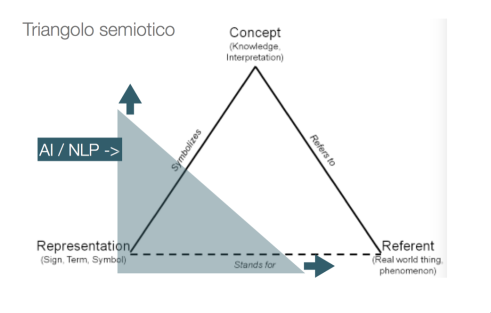
\includegraphics[scale=0.6]{02/tr.png}
    \caption{Triangolo semiotico.}
    \label{fig:semtr}

  \end{figure}

\cor{Concetto}{Corrisponde a ciò che si ha in mente senza utilizzare una convenzione.}

\cor{Rappresentazione}{Si utilizza un simbolo convenzionale per comunicare il concetto.}

\cor{Referente}{Un'istanza del concetto, ossia un elemento nel mondo reale.}

\nt{Per esempio il concetto di "gatto" in italiano e in inglese è lo stesso, ma la sua rappresentazione cambia (gatto/cat). Il referente è un qualsiasi gatto.}

\qs{}{Dove si collocano IA e NLP in questo triangolo e in quale direzione si muovono?}

L'unico punto da cui si può partire è la rappresentazione perché nessun sistema informatico può prendere un concetto direttamente dalla nostra testa. Dall'insieme di testi presenti nel web si cerca di creare una concettualizzazione e si cerca di muoversi verso i referenti. 

\section{Multilinguismo e Granularità}

\subsection{Multilinguismo}

Una delle sfide del NLP moderno è quella di trattare una pluralità di lingue, il ché è un'arma ha doppio taglio: è più difficile, ma fornisce molte più sfumature di significato. Analizzare un testo in più lingue permette di:

\begin{itemize}
  \item Capire quali sono le informazioni semantiche più importanti, più certe o maggiormente condivise. 
  \item Migrare informazioni semantiche da una lingua all'altra.
\end{itemize}

\clm{}{}{
  Possibili problemi:
  \begin{itemize}
    \item I testi in lingue rare sono molto difficili da gestire, anche considerando che la maggior parte del web e dei testi scientifici è in inglese. 
    \item Le lingue hanno sfumature che non possono essere tradotte direttamente.
  \end{itemize}
}

\subsection{Granularità}

\paragraph{La Granularità può essere a livello di:}

\begin{itemize}
  \item \fancyglitter{Parola:} complessità elevata. 
  \item \fancyglitter{Chunk:} composizione di parole (e.g. aggettivo + nome). 
  \item \fancyglitter{Discorso:} come per i chatBOTs. 
  \item \fancyglitter{Documento:} sistemi di sommarizzazione:
    \begin{itemize}
      \item Estrattivi: estrapolano dal testo le parti più significative. 
      \item Astrattivo: generano nuove frasi a partire dal documento. 
    \end{itemize}
  \item \fancyglitter{Collezione di documenti:} estrapolare gli argomenti principali (topic modelling).
\end{itemize}

\section{Costruzione del Significato}

\subsection{Pustejovsky}

Pustejovsky propose una teoria chiamata \fancyglitter{generative lexicon} che utilizza una struttura basata su:

\begin{itemize}
  \item \fancyglitter{Argument Structure:} per esprimere il legame tra sintassi e semantica del concetto. In altre parola come mappare ciò che si vuole esprimere su un concetto mediante l'uso di lettere, parole e grammatica. 
  \item \fancyglitter{Event Structure:} per esprimere tutti i tipi di evento che coinvolgono quel concetto. 
  \item \fancyglitter{Qualia Structure:} per esprimere come sono definite le caratteristiche (qualia) di un concetto.
  \item \fancyglitter{Inheritance Structure:} per collocare il concetto all'interno di una tassonomia per inferirne il significato.
\end{itemize}

Pustejovsky sostiene che per poter ragionare semanticamente in maniera precisa e completa abbiamo bisogno di formalizzare tutte queste strutture. 

\dfn{Qualia}{
  La qualia ha 4 ruoli:
  \begin{itemize}
    \item Costitutivo: esprime la parte di composizione del soggetto, riguarda il peso, la dimensione e le parti che lo compongono. 
    \item Formale: esprime le caratteristiche che distinguono un concetto dagli altri dello stesso dominio. 
    \item Telico: l'obiettivo o la funzione del concetto, il suo ruolo comportamentale.
    \item Agentive: tutte le entità (spesso umane) che rappresentano l'origine del concetto.
  \end{itemize}
}

\nt{Si tratta di una teoria formale in cui si assegna a ciascun elemento un ruolo e una struttura in base ai concetti definiti da Pustejovsky. In questo modo ogni frase può essere analizzata in modo formale. Il problema di questa teoria e la sua complessità che la rende difficile da implementare.}

\subsection{Hanks}

Patrick Hanks enuncio una teoria del significato più semplice di quella di Pustejovsky: la \fancyglitter{teoria delle valenze}. Questa teoria si basa sul concetto che il verbo sia la radice del significato: non esiste un'espressione di significato senza un verbo.

\dfn{Valenza}{
  La valenza (fig: \ref{fig:val}) è la cardinalità degli oggetti che compongono la struttura di cui il verbo è la radice. Un verbo può essere transitivo o intransitivo a vari livelli.
    
}

\begin{figure}[h]
    \centering
    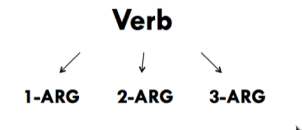
\includegraphics[scale=0.6]{02/valenze.png}
    \caption{Valenze.}
    \label{fig:val}
\end{figure}

\nt{Ogni valenza rappresenta un numero di argomenti chiamati slot e ogni possibile valore che possono assumere e chiamato filler.}

\paragraph{Dati un verbo e una valenza si hanno (fig: \ref{fig:val2}):}

\begin{itemize}
  \item \fancyglitter{Collocazione:} la combinazione di tutti i possibili filler. 
  \item \fancyglitter{Semantic Type:} delle macrocategorie che servono per raggruppare i vari filler.
\end{itemize}

\begin{figure}[h]
    \centering
    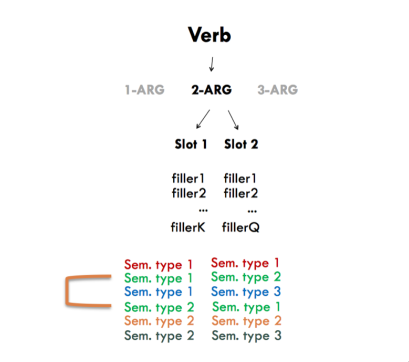
\includegraphics[scale=0.6]{02/val.png}
    \caption{Le due righe in verde rappresentano una valenza sintattica.}
    \label{fig:val2}
\end{figure}

\qs{}{Quali sono i Semantic Type? Quale deve essere il grado di generalizzazione?}

\begin{itemize}
  \item Non sempre si hanno sufficienti dati per tutte le parole, alcune sono rare e difficili da analizzare. 
  \item I termini nei dati possono non sovrapporsi anche se sono simili. 
\end{itemize}





